\documentclass[a4paper,10pt]{article}
\usepackage[utf8]{inputenc}
\usepackage{graphicx}        % standard LaTeX graphics tool
\usepackage{amsmath}
\usepackage{amsfonts}
\usepackage{framed}
\usepackage{tcolorbox}
\tcbuselibrary{breakable}
\DeclareMathOperator{\E}{\mathbb{E}}
\DeclareMathOperator{\sensor}{\mathbf{s}}
\DeclareMathOperator{\world}{\mathbf{w}}
% Title Page
\title{Notes on Quaternion-based Extended Kalman Filter Orientation Estimation}
\author{Jorhabib Eljaik Gomez}
\date{}


\begin{document}
\maketitle

% \chapter*{Quaternion-based Methods for Orientation Estimation.}
% \label{chap:methods}

\section{Initial Considerations}
In all of the followig versions of the filter, we will assume the following:

\begin{itemize}
 \item $x$ - State vector.
 \item $q$ - Quaternion vector.
 \item The process to be estimated is random and can be modeled as:
 $x_{k+1} = \phi_k x_k + w_k$.
 \item The measurement (observation) of the process respects the linear relationship $z_k = H_k x_k + v_k$.
 \item An initial estimate of the process at some time $t_k$ is available. This prior estimate is denoted $\hat{x}^{-}_k$.
 \item  The error covariance matrix associated with $\hat{x}^{-}_k$ is known, which corresponds to $P^{-}_k = E[e^{-}_k {e^{-}}^T_k]$ where $e^{-}_k$ is the \textbf{estimation error} defined as ${e^{-}}_k = x_k - \hat{x}^{-}_k$.
\end{itemize}

Where:
\begin{list}{variables}{}
 \item $x_k (n \times 1)$ process state vector at time $t_k$
 \item $\phi_k (n \times n)$ matrix relating $x_k$ to $x_{k+1}$ in the absence of a forcing function (no input).
 \item $w_k (n \times 1)$ noise vector with known covariance structure.
 \item $z_k (m \times 1)$ vector measurement at time $t_k$
 \item $H_k (m \times 1)$ matrix giving the (noiseless) linear relationship between the measurement and the state vector at time $t_k$
 \item $v_k (m \times 1)$ measurement error
\end{list}

Covariance matrices for the $w_k$ and $v_k$ vectors at time $t_k$ are given by $Q_k$ and $R_k$.

\subsection{Kalman Filter}
\label{sec:KalmanFilter}
Here goes a summarized explanation of the Kalman Filter.
\begin{figure}[!ht]
 \centering
 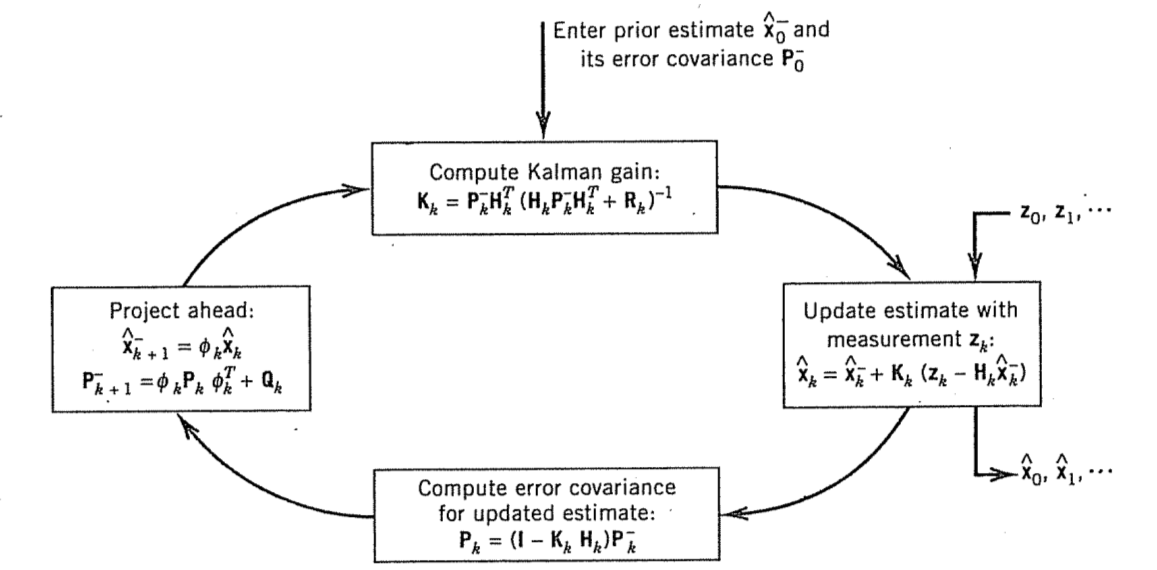
\includegraphics[width=0.9\textwidth]{./fig/kalman_loop.png}
 % kalman_loop.png: 1157x570 pixel, 72dpi, 40.82x20.11 cm, bb=0 0 1157 570
 \caption{Kalman filter algorithm. Extracted from Introduction to Random Signals and Applied Kalman Filtering.}
 \label{fig:kalmanLoop}
\end{figure}

\subsection{Sensors Calibration}
This is a very delicate and important issue that needs to be addressed. Good summarized information can be found in \cite{Cucu2012} and the selected choice described here.

\newpage

\section*{Quaternion-based Kalman Filter. A Detailed Description.}
by Jorhabib Eljaik G. \newline \\
The goal of this Kalman Filter is to estimate the orientation of the Earth-fixed (world) reference frame\footnote{Defined as a right-handed co-ordinate system with the positive $x$ axis pointing to the local magnetic North, positive $z$ pointing up and $y$ according to the right handed system} $\{\world\}$ with respect to the body (sensor) reference $\{\sensor\}$ in the quaternion representation (in radians), i.e.~$q^{\sensor}_{\world}$. This representation is chosen to avoid the singularities that may be incurred when using local parametrizations such as Euler Angles (e.g. when the pitch approaches $\pm90^{\circ}$). The usage of this representation however, complicates a bit the mathematical description of the filter. In this report we present a detailed description of a proper yet fairly simple implementation. 
We start with a simplified version of the filter where only a triad of gyroscopes and accelerometers will be used along with a simple model of the process representing solely the orientation to be estimated. In this way, the state of the Kalman Filter will be the quaternion-based orientation of the world in the sensor reference frame $\{\sensor\}$, i.e.
\begin{equation}
  x = q^{\sensor}_{\world}
\end{equation}
Where $q = [q_1 \quad q_v]$, $q_1 \in \mathbb{R}$, $q_v \in \mathbb{R}^3$ and $||q|| = 1$. Our ground truth will be the estimate of the MTx inertial measurement unit (IMU) which is also used to acquire sensor readings (accelerometer and gyro). This estimate however is expressed in $\{\world\}$, so the conjugate of our final estimate is what's actually compared. It is known that the estimation done in the MTx is also a Kalman-filter-based one (as stated in the documentation) and uses some of the assumptions present in this work.

\begin{figure}[ht!]
 \centering
 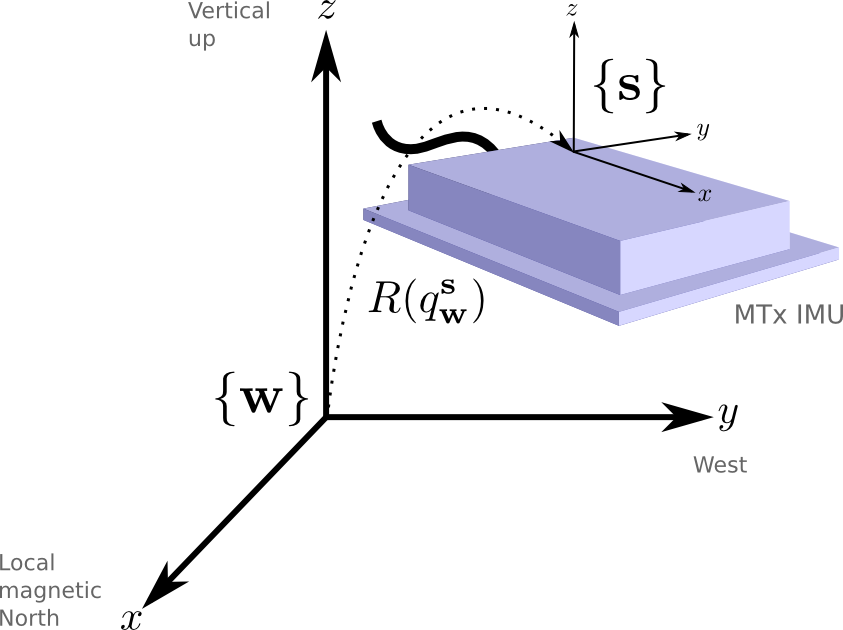
\includegraphics[width=0.5\textwidth]{./fig/MixCoordSys.png}
 % MixCoordSys.png: 365x315 pixel, 90dpi, 10.30x8.89 cm, bb=0 0 292 252
 \label{fig:coordsys}
 \caption{Earth-fixed (world) reference frame $\{\world\}$ and local sensor reference frame $\{\sensor\}$. $R(q^{\sensor}_{\world})$ denotes the quaternion-based rotation matrix that rotates the world reference frame $\{\world\}$ into $\{\sensor\}$. }
\end{figure}


\subsection{\textbf{Discrete Time Process Model}} 
[$x_{k+1} = Ax_k + w_k$]. This model is obtained starting off the continuous time equations relating the quaternion orientation with its derivative resulting in the following differential equation \cite{Trawny2005}: 
 \begin{equation}
  \dot{q}^{\sensor}_{\world}(t) = \frac{1}{2}\Omega(\omega^{\sensor}(t))q^{\sensor}_{\world}(t)
  \label{Eq:diffEq}
 \end{equation}
 From now on, let us forget about the super and subscript identifying the reference frames for this quaternion for the sake of clarity, and let us work out Eq.~\ref{Eq:diffEq} in order to obtain the more cannonical equation of the process model. In the previous equation $\omega$ is the \textbf{actual} angular velocity in body coordinates. The relationship between this angular velocity and the one measured by a gyroscope $\omega^m$ with zero-mean normal additive noise $\epsilon_k$ at time $k$ is given by:
  \begin{equation}
   \omega^m_k = \omega_k + \epsilon_k
  \end{equation} 
  
  Let us then call $\Omega(\omega)$ the ``derivative matrix'' which appears in the multiplication of a matrix by a quaternion and has the same structure:
  \begin{equation}
  \Omega(\omega)=
     \left[\begin{array}{cc}
         0      & -\omega^T  \\
       \omega   & -S(\omega)
    \end{array}  \right]
  \end{equation}

  The discrete-time solution to Eq.~\ref{Eq:diffEq} is known to be: 
 \begin{equation}
  q_{k+1} = \Phi_k q_k
  \label{Eq:transitionEq}
 \end{equation}
 Under the assumption that $\omega$ is constant over the integration time ($T_s$), thus making $\Omega$ independent of time, the differential equation becomes time-invariant and a closed form solution can be obtained resulting in the so-called ``zeroth order quaternion integrator" \cite{Trawny2005}, thus: 
 \begin{equation}
  \Phi_k = \text{exp}\left( \frac{1}{2}\Omega({\omega})T_s \right)
 \end{equation}
  Using the Taylor expansion of this matrix exponential along with the power properties of matrix $\Omega(\omega)$, you get the common Taylor series expansions of the $sine$ and $cos$ functions and taking the first order approximation (as $\omega \rightarrow 0$) we finally obtain \cite{Trawny2005}:
  \begin{equation}
   \Phi_k = I_{4\times4} + \frac{T_s}{2}\Omega({\omega})
  \end{equation}
  In this simplified case of the filter, since we are not estimating $\omega$, but measuring it with the gyroscope which is subject to error and bias, the transition matrix that uses $\omega_m$ instead of $\omega$ will differ from $\Phi_k$ by $\Delta\Phi_k$, that is: 
  
  \begin{equation}
   \Phi^m_k = \Phi_k + \Delta\Phi_k
   \label{Eq:measuredPhi}
  \end{equation}
  
  $\Delta\Phi_k$ is called the Error Matrix which according to \cite{Choukroun2003} can be expressed as its matrix power series first order term only, or from the first order approximations of $\Phi^m_k$ and $\Phi_k$, such that:
  \begin{align}
   \Phi^m_k - \Phi_k &= (I_{4\times4} + \frac{1}{2}\Omega(\omega^m_k)T_s) - (I_{4\times4} + \frac{1}{2}\Omega({\omega_k})T_s) \\
                     &= \frac{1}{2}\Omega(\omega^m_k - \omega_k)T_s \\
                     &= \frac{1}{2}\Omega(\epsilon_k)T_s = E_k T_s
  \end{align}
  Where $\epsilon_k$ is the gyro measurement noise vector, thus: 
  \begin{equation}
   \Delta{\Phi_k} \simeq E_k T_s
  \end{equation}
  
  Where 
  \begin{equation}
  E_k = \frac{1}{2}\left[ \begin{array}{cc}
                           0      & -\epsilon^T_k  \\
                           \epsilon_k & -S(\epsilon_k) \\
                          \end{array}  \right]
  \end{equation}
  
  And $S(\epsilon_k)$ the skew-symmetric matrix:
  \begin{equation}
    S(\epsilon_k) = \left[ \begin{array}{ccc}
                                0       &  -\epsilon_{k_3} & \epsilon_{k_2}  \\
                          \epsilon_{k_3}  &        0       & -\epsilon_{k_1} \\
                          -\epsilon_{k_2} &   \epsilon_{k_1} &       0       
                         \end{array} \right]
  \end{equation}
  
  Hence, from Eq.~\ref{Eq:measuredPhi}
  \begin{align}
   \Phi_k &= \Phi^m_k - \Delta \Phi_k \\
   \Phi_k &= \Phi^m_k - E_k T_s
  \end{align}
  Substituting in Eq.~\ref{Eq:transitionEq}
  \begin{align}
   q_{k+1} &= \Phi_k q_k \\
   q_{k+1} &= (\Phi^m_k - E_k T_s)q_k \\
   q_{k+1} &= \Phi^m_k q_k - T_s E_k q_k \label{Eq:transitionEq2}
  \end{align}
  In \cite{Choukroun2003} it is explained how the term $E_k q_k$ can be further expanded taking advantage of the properties of the matrix $E_k$, which when pre-multiplying a quaternion respects the following property ($\Omega(\omega)$ and $E_k$ have the same structure!):
  
  \begin{tcolorbox}
   Given $\Omega(x) = \left[\begin{array}{cc}
                               0   & -x^T \\
                               x   & -S(x)
                            \end{array}\right]$
  and $\Xi(q) = \left[\begin{array}{c}
                   -q^T_v \\
                   q_1 I_{3\times3} + S(q_v)
                 \end{array}\right]$ \newline
    \begin{equation}
     \centering
     \Omega(x)q = \Xi(q)x
     \label{Eq:propertyXi}
    \end{equation}
    \begin{center}
      $\forall~x \in \mathbb{R}^3$
    \end{center}
  \end{tcolorbox}

  Thus, Eq.~\ref{Eq:transitionEq2} can be further expressed as:
  \begin{equation}
   q_{k+1} = \Phi^m_k q_k - \frac{T_s}{2} \Xi(q_k)\epsilon_k
  \end{equation}
  Taking $x = \epsilon$ and $q=q_k$.
  Finally, the \textbf{Process Model} is: 
  \begin{tcolorbox}
   \begin{equation}
    x_{k+1} = q_{k+1} = \Phi^m_k q_k + w_k
    \label{Eq:processModel}
   \end{equation}
   Where: 
   \begin{align}
    \Phi^m_k &= I_{4\times4} + \frac{T_s}{2}\Omega(\omega^m_k) \\
    w_k      &= -\frac{T_s}{2}\Xi(q_k)\epsilon_k \label{Eq:noiseVecEq}\\
    \Xi(q_k) &= \left[\begin{array}{c}
                -q^T_v \\
                q_1 I_{3\times3} + S(q_v)
               \end{array}\right]
   \end{align}
   The zero-mean gyro noise vector $\epsilon_k$ is normally distributed, i.e. $\epsilon \sim \mathcal{N}(0,\sigma_g)$
   \begin{equation}
    \Sigma^{g}_k = \sigma^2_{g} I_{3\times3}
   \end{equation}
   With process covariance matrix given by:
     \begin{equation}
      Q^w_k = E(w_k w^T_k) = \left(\frac{T_s}{2}\right)^2 \Xi_k \Sigma^{g}_k \Xi^T_k
     \end{equation}
  \end{tcolorbox}
  
  Remember that $T_s$ must be kept small, as well as $\epsilon_k$ since these assumptions allowed for the approximation of $\Delta \Phi_k$, the Error Transition Matrix first order approximation. 
  The fact that the process noise vector $w_k$ is state dependent can be addressed by substituting $q_k$ in Eq.~\ref{Eq:noiseVecEq} with the most recent estimate as done in \cite{Choukroun2003} or \cite{Sabatini2006}.

  \subsection{Measurement Model}
  [$z_{k} = h(x_{k+1}) + v_{k}$]. This model is constituted by the accelerometer only, neglecting its bias and scaling factors or body acceleration. The latter assumption is also done in many commercial IMUs as the one used to compare our results. The measurement model in the body frame:
  
  \begin{equation}
   z_{k} = h(q^{\sensor}_{\world{k+1}}) + v_{k}
  \end{equation}
   \begin{tcolorbox}
   \begin{equation}
    z_{k} = R(q^{\sensor}_{\world{k+1}}) g^{\world} + v_{k} 
   \end{equation}
   \label{Eq:measEq}
   \end{tcolorbox}
  
  Where $R(q^{\sensor}_{\world_{k+1}})$ is the rotation matrix representing the orientation of the sensor reference frame with respect to the world frame. This rotation matrix is a function of the quaternion orientation. $g^{\world}$ is the gravity vector (as it would be measured by the accelerometer) in Earth coordinates and is considered constant and equal to $[0~0~9.8]^T$. The covariance matrix of the measurement model is assumed constant and equal to:
  \begin{equation}
   \Sigma^{a}_{k} = \sigma^2_a I_{3\times3}
  \end{equation}
  
  \subsection{Filter design}
  The measurement model described by Eq.~\ref{Eq:measEq} is non-linear in $q$. To fully describe the filter we further need to linearize $h(q^{\sensor}_{\world_{k+1}})$. Notice that the process model given by Eq.~\ref{Eq:processModel} is already linear in $q$.
  
  \begin{figure}[ht!]
 \centering
 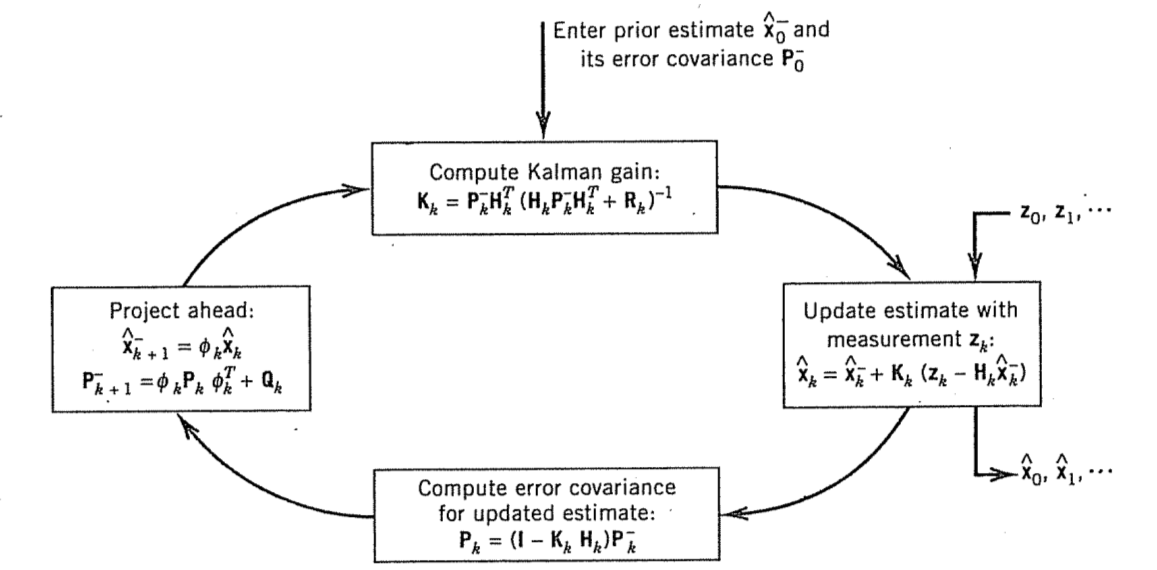
\includegraphics[width=\textwidth]{./fig/kalman_loop.png}
 % kalman_loop.png: 1157x570 pixel, 72dpi, 40.82x20.11 cm, bb=0 0 1157 570
 \caption{Recursive Kalman Filter. This is only for reference on the linear Kalman Filter. The notation used here does not reflect the one used in this notes. Extracted from \cite{Grover1996}}
 \label{fig:kalmanLoop}
\end{figure}

  To linearize Eq.~\ref{Eq:measEq} we proceed to compute the Jacobian of $h(q)$, evaluated at the most recent estimate of $q$. Let us recall here that $R(q^{\sensor}_{\world})$ can be expressed in terms of the quaternion as:
  \begin{equation}
   R(q^{\sensor}_{\world}) = \left[\begin{array}{ccc}
               2q^2_1-1+2q^2_2 & 2q_2q_3 - 2q_1q_4 & 2q_2q_4 + 2q_1q_3 \\
               2q_2q_3+2q_1q_4 & 2q^2_1-1+2q^2_3 & 2q_3q_4-2q_1q_2 \\
               2q_2q_4-2q_1q_3 & 2q_3q_4+2q_1q_2 & 2q^2_1-1+2q^2_4
              \end{array}\right]
  \end{equation}

  The observation matrix is then defined by the following Jacobian:
  \begin{align}
   H_{k+1} &= \left.\frac{\partial h}{\partial q} \right|_{x_{k+1|k}} \\
           &= \left.\frac{\partial}{\partial q} R(q^{\sensor}_{\world}) g^{\world}\right|_{x_{k+1|k}}
  \end{align}

  Where
  \begin{equation}
  \frac{\partial}{\partial q} R(q^{\sensor}_{\world}) =\left[\begin{array}{cccc}
                                                \frac{\partial}{\partial q_1} R(q) & \frac{\partial}{\partial q_2} R(q) & \frac{\partial}{\partial q_3} R(q) & \frac{\partial}{\partial q_4} R(q)
                                               \end{array}\right]
  \end{equation}

  with
  \begin{align}
   \frac{\partial}{\partial q_1} R &= 2\left[ \begin{array}{ccc}
                                               2q_1 & -q_4 &  q_3 \\
                                               q_4  & 2q_1 & -q_2 \\
                                               -q_3 & q_2  & 2q_1
                                              \end{array}\right] \\
   \frac{\partial}{\partial q_2} R &= 2\left[ \begin{array}{ccc}
                                               2q_2 & q_3 & q_4 \\
                                               q_3  & 0   & -q_1 \\
                                               q_4  & q_1 & 0
                                              \end{array}\right] \\
   \frac{\partial}{\partial q_3} R &= 2\left[ \begin{array}{ccc}
                                               0    & q_2  & q_1 \\
                                               q_2  & 2q_3 & q_4 \\
                                              -q_1  & q_4  & 0
                                              \end{array}\right] \\
   \frac{\partial}{\partial q_4} R &= 2\left[ \begin{array}{ccc}
                                               0    & -q_1  & q_2 \\
                                               q_1  &  0    & q_3 \\
                                               q_2  & q_3   & 2q_4
                                              \end{array}\right]                                               
  \end{align}

  At this point we have all the elements necessary to implement an Extended Kalman Filter with linearized measurement equations. The C++ implementation of this filter has been done with a modified version of the open source \emph{Bayesian Filtering Library} (BFL).
  
 \newpage

\section{Estimating Accelerometer Bias}
Accelerometers and gyroscopes are subject to scaling factors, bias and errors.

\section{Multiplicative Kalman Filter}
The Kalman Filter explained in Section \ref{sec:KalmanFilter} is known as a \emph{Direct Kalman Filter} 


\section{Simplified Version Using the QUaternionESTimator algorithm (QUEST)}
\label{sect:questSection}
An alternative to the linearization of the accelerometer measurement equation is that of fusing the accelerometer and magnetometer measurement into a single one through an efficient statistical attitude determination method called QUEST, which stands for QUaternion ESTimator. The basic idea is that if two orientation observations are available, this information can be joint together using a statistical method. Suppose we have a set of of $N$ unit vectors $\hat{z}_k$, for which we have the mathematical model	 that relates their sensor measurement in the inertial ${i}$ frame to the body frame ${b}$ through a rotation matrix $R^b_i$ as:

\begin{equation}
 z_{kb} = R^b_i z_{ki}
\end{equation}

This set of equations is overdetermined when having two or more readings. For this reason, we want to find a solution for $R^b_i$ that minimizes the overall error for all vectors. The classical way to state this problem is as an optimization one that minimizes the sum of the squared errors for each vector measurement. Thus, the loss function can be expressed as:

\begin{equation}
 J(R^b_i) = \frac{1}{2}  \sum^{N}_{k=1}  w_k \left| z_{kb} - R^b_i z_{ki} \right|^2 
\end{equation}

Where $J$ is the loss function to be minimized, $k$ is the index for observations (measurements) $z_{k}$ is the $kth$ vector being measured, $z_{kb}$ is the matrix of measured components in the body frame and $z_{ki}$ the matrix of components in the inertial frame \cite{HallNotes2003}. The previous loss function is also known in literature as Wahba's loss function. 

Depending on how noisy measurements are, the harder it becomes to minimize this loss function. 

QUEST is just one efficient way to perform this minimization and will be described next. Many spacecraft attitude systems use this method to fuse the unit vector giving the direction to the sun or a star and the unit vector in the direction of the Earth's magnetic field. In this particular implementation we intend to do the same, with the gravity vector given by the accelerometer and the Earth's magnetic field direction provided by the magnetometer.

\section{Bayesian Interpretation of the Kalman Filter}
The Kalman Filter can be seen as a special case of the sequential state estimation problem in iterative Bayesian filtering. In recursive Bayesian estimation, two assumptions are used to derive the recursive Bayesian filter: i) The state follows a first-order Markov process, meaning $p(x_n | x_{0:n-1}) = p(x_n | x_{n-1})$, ii) The observations are independent of the given states. From Bayes rule it can be obtained that the \textbf{conditional pdf} of $x_n$  is:

\begin{equation}
 p(x_n|y_{0:n}) = \frac{p(y_n|x_n)p(x_n|y_{0:n-1})}{p(y_n|y_{n-1})}
\end{equation}

In the previous equation the posterior probability is described by three terms:
\begin{itemize}
 \item \textbf{Prior:} $p(x_n|y_{0:n-1})$ and is also a function of the transition probability $p(x_{n+1}|x_n)$ (or $p(x_{n}|x_{n-1})$) which is further characterized by the transition matrix $F$ from the formulation of the discrete dynamic state-space problem. 
 \item \textbf{Likelihood:} $p(y_n|x_n)$ which is characterized by a measurement equation $y_n = g(x_n, v_n)$ where $v_n$ is measurement noise (or its measurement matrix $H_n$).
 \item \textbf{Evidence:} $p(y_n|y_{0:n-1})$
\end{itemize}

Kalman Filtering can be reduced to a Maximum A Posteriori (MAP) solution to
\begin{equation}
 \left.\frac{\partial \log p(x_n|y_{0:n})}{\partial x_n}\right\vert_{x_n = \hat{x}^{MAP}} = 0
\end{equation}

after calculating the means and covariances of the previously listed terms, i.e.
\begin{equation}
\begin{aligned}
 E[y_n|x_n]        &= G_n x_n\\
 Cov[y_n|x_n]       &= \Sigma_v\\
 E[x_n|y_{0:n-1}]   &= Fx_{n-1}\\
 Cov[x_n|y_{0:n-1}] &= Cov[x_n - \hat{x}_{n|n-1}]
\end{aligned}
\end{equation}


And pdfs:

\begin{align}
 p(y_n|x_n)       &= A_1 \exp(-\frac{1}{2}(y_n - G_n x_n)^T \Sigma^{-1}_v (y_n - G_n x_n)) \\
 p(x_n|y_{0:n-1}) &= A_2 \exp(\frac{1}{2}(x_n - \hat{x}_{n|n-1})^T \times P^{-1}_{n,n-1}(x_n - \hat{x}_{n|n-1}))\\
\end{align}

We can now obtain an expression for the posterior $p(x_n|y_{0:n})$ as:
\begin{multline}
 p(x_n|y_{0:n}) \propto A \exp\left(\frac{1}{2} (y_n - G_n x_n)^T)\Sigma^{-1}_v (y_n - G_n x_n) \right.\\
		\left.- \frac{1}{2}(x_n - \hat{x}_{n|n-1})^T P^{-1}_{n,n-1}(x_n - \hat{x}_{n|n-1}\right)
\end{multline}

Where $A_1 = 2\pi^{-N_y/2}|\Sigma_v|^{-1/2}$, $A_2 = 2\pi^{-N_x/2}|P_{n,n-1}|^{-1/2}$ and $A=A_1 A_2$. 
For more details on these derivations and further references please refer to \cite{Chen2003}.

\section{Notes on BFL}

\section{Performing orientation estimate for iCub's feet}
\section{Installing the skin on the iCub}
\subsection{Ethernet-based robot}
Initial experiments are being done with the right foot only, for which the following description will concern just that foot.
\begin{itemize}
  \item Assuming local (experimental) changes, \texttt{cd} into \texttt{ICUB\_DIR/share/iCub/} \texttt{ICUB\_DIR/share/iCub/robots/iCubGenova02/hardware/skin}. In the file \texttt{right\_leg-ems11-inertial\_mtb.xml} in group \texttt{GENERAL} set \\ \texttt{param name=enabledGyroscopes} to \texttt{r\_foot\_1} and \texttt{r\_foot\_2}.\\
  \item The port that will be opened can be set in \texttt{ICUB\_DIR/share/iCub/ro\-bots/iCubGeno\-va02/wrappers/skin}. By default it is \texttt{right\_leg/iner\-tialMTB}
  \item In the port previously reported you will find readings from all accelerometers and gyroscopes that have been activated. The ID number for \texttt{r\_foot\_1} is $32$ (8 + \texttt{eoas\_inertial\_pos\_offsetright}) and for \texttt{r\_foot\_2} is $33$ (9 + \texttt{eoas\_inertial\_pos\_offsetright}). These numbers can be obtained from the \texttt{eOas\_inertial\_position\_t} enumeration type in which \texttt{eoas\_inertial\_pos\_offsetright} is $24$ while \texttt{eoas\_inertial\_pos\_offsetleft} is $0$
\end{itemize}

\subsection{Hardware}
Two multimodal skin boards usually used in the palms of the robot have been used for this experiment.


\newpage
\bibliographystyle{plain} 
\bibliography{references}

\end{document}          
